\chapter{Introduction}

\textit{There's an infinity of things that have never been done before, and most of those things are not worth doing.} -- Jeremy Fox, \textit{Dynamic Ecology (2016)}~\cite{fox_how_2016}

\selectlanguage{french}
\section*{Résumé en français}

Dans cette section... (env. 1-2 pages)
\selectlanguage{english}

\begin{center}
\noindent\rule{4cm}{0.1pt}
\end{center}

\section{Context}
\label{sec:context}

\subsection{Self-replication is a resource allocation problem}

At every moment of our lives, we are surrounded by billions of microscopic organisms.
They sustain themselves by collecting energy from their environment, in the form of organic matter, highly reactive chemicals, or light~\cite{madigan_biology_2006,schaechter_microbe_2006}.
While most of our cells are kept in a stable and friendly internal environment (temperature, oxygenation, nutrient abundance, ...), microorganisms have evolved to constantly adapt their physiology to strongly variable environments.
Not without a certain success, because microbes have been found to survive almost everywhere, sometimes in the strangest places that were initially thought unsuitable for life~\cite{rothschild_life_2001,nicholson_transcriptomic_2012,madigan_biology_2006,schaechter_microbe_2006}.
Such ubiquity translates a strong potential for adaptation.
Even the model organism \textit{Escherichia coli}, a bacteria first isolated from our intestinal track, is capable of growing on dozens of different carbon sources through changes in the expression of thousands of genes\cite{zimmer_microcosm:_2009}.

Microorganisms, along with all living cells, are mainly constituted of polymers (DNA, RNA, Proteins) made of many repeated sub-units (nucleotides, amino acids).
The information about their sequences is stored in the form of genes on the DNA.
Gene expression is the process by which this information is used in the synthesis of a functional final product (protein or RNA).
The gene expression machinery (itself constituted of RNA and proteins) synthesizes the gene products after binding to gene promoters, which are target sequences on the DNA.
In a given cell, they are roughly as many different target sequences as genes, which ensures that not all products are synthesized at the same rate.
Furthermore, some of these products specifically bind some promoters and stimulates or represses the promoter activity, hence, the gene expression.
They are called transcription factors and allow, among other mechanisms, the regulation of cell composition.

The reorganization of gene expression controls the abundance of enzymes and ribozymes that catalyzes the biochemical reactions allowing the cell to perform different functions.
For instance, assimilating a given nutrient involves the synthesis of the corresponding uptake protein and of the metabolic enzymes converting the nutrients into reductive power, nucleotides and amino acids~\cite{schaechter_microbe_2006}.
These precursors are then used to produce new macromolecules, closing the loop of self-replication.
In order to optimize the overall process in different environmental conditions, the cell must adjust the abundance of every enzyme involved in this network of biochemical reactions.
By doing so, the cell actually resolves a resource allocation problem, where a common wealth (precursors) has to be distributed over thousands of potential beneficiaries (proteins and other macromolecules).

\subsection{Optimizing biomass production yields a competitive advantage}

Which resource allocations are optimal for a living cell?
Systems capable of Darwinian evolution sustain themselves on the long term by \textit{fitting} to their environment.
Living cells with the best \textit{fitness} are more likely to survive, replicate, and through long-term competition, eliminate their siblings.
The optimization criteria that quantitatively measure \textit{fitness} are called \textit{fitness factors}.
Whether they apply at the species, the population, the organism, or even the gene level has long been debated~\cite{dawkins_selfish_1976}.
An optimal resource allocation would be a gene expression scheme that maximizes the fitness factors.
But since fitness factors have to take into account the ability to survive, reproduce, and compete with other organisms in a given (sometimes changing) environment, they are often context-dependent and highly difficult to identify.

For this reason, there is no consensus about what constitute the main fitness factors of microorganisms.
Competition for common resources seems to favor the maximization of offspring, in the sense that a replicator with more descendants will outnumber its competitors in the long term~\cite{dawkins_selfish_1976}.
It is unclear, however, how this general principle translates into their physiological behaviors.
For instance, the use of genome-scale metabolic network models have shown that the metabolism maximizes the production either of biomass or available energy (ATP) depending on the environmental condition~\cite{schuetz_systematic_2007}.
But we can also found different strategies when the biomass production is at play.
Bacteria can either optimize their production yield (taking its time to make the most of the nutrient) or their production rate (growing quickly while wasting part of the nutrient potential), the later being favored in fluctuating or poor environments~\cite{frank_tradeoff_2010,maclean_tragedy_2008}, a result that has also been confirmed in yeast~\cite{schuster_maximization_2008}.
Overall, it seems that cell optimality drifts in a multidimensional space and involves making several trade-offs that strongly depend on the environmental context~\cite{schuetz_multidimensional_2012}.

Nevertheless, numerous studies have shown that considering growth rate maximization confers a good predictive power of microorganism physiology.
When cultivated in minimal medium with acetate or succinate, \textit{Escherichia coli} uptake rates are correctly predicted by assuming that the metabolic network operates in a mode that maximizes growth rate~\cite{edwards_silico_2001}.
This result is not general though, and depends on the carbon source and strain used~\cite{ibarra_escherichia_2002}.
But even in those cases, the metabolic networks evolve rapidly towards growth-rate maximization if a constant nutrient-providing environment is maintained~\cite{ibarra_escherichia_2002}.
The mutants obtained present modications in the regulation of the synthesis of metabolic enzymes~\cite{lewis_omic_2010}, indicating that not only the efficiency of the enzymes is affected, but also their abundance and thus the cellular composition.
Overall, with the currently available knowledge and its limitations (discussed in section~\ref{chap:discussion}), growth-rate maximization sounds like a rational choice to understand the growth strategies of microorganisms~\cite{molenaar_shifts_2009}.

\subsection{Growth laws are universal strategies employed by microorganisms}

One of the first attempt to formalize microorganism physiology into elegant, fundamental laws was the discovery of Monod's law more than sixty years ago~\cite{monod_growth_1949}.
This empirical relationship states that the growth rate $\mu$ [\texttt{div.h\textsuperscript{-1}}] of \textit{Escherichia coli} is a hyperbolic function of the concentration of the limiting nutrient $C$ [\texttt{mol.L\textsuperscript{-1}}], such that
\begin{equation}
\label{eq:monod_law}
\mu = \mu_K \frac{C}{K_C + C}
\end{equation}
with $\mu_K$ and $K_C$ two constants depending on the quality of the nutrient (Fig~\ref{fig:monod_law}).
It is remarkable that the growth rate, a parameter that depends on the use and production of thousands of proteins, can be so easily predicted by a simple relation.
What is even more remarkable is that this relation is rather universal.
Despite some adjustments (the Droop model being a well-known example~\cite{droop_thoughts_1973}), the relation holds for most microorganisms: the growth rate increases with the abundance of the limiting nutrient, up to a point beyond which they cannot grow any faster~\cite{koch_why_1988}.

\begin{figure}[tb]
\centering
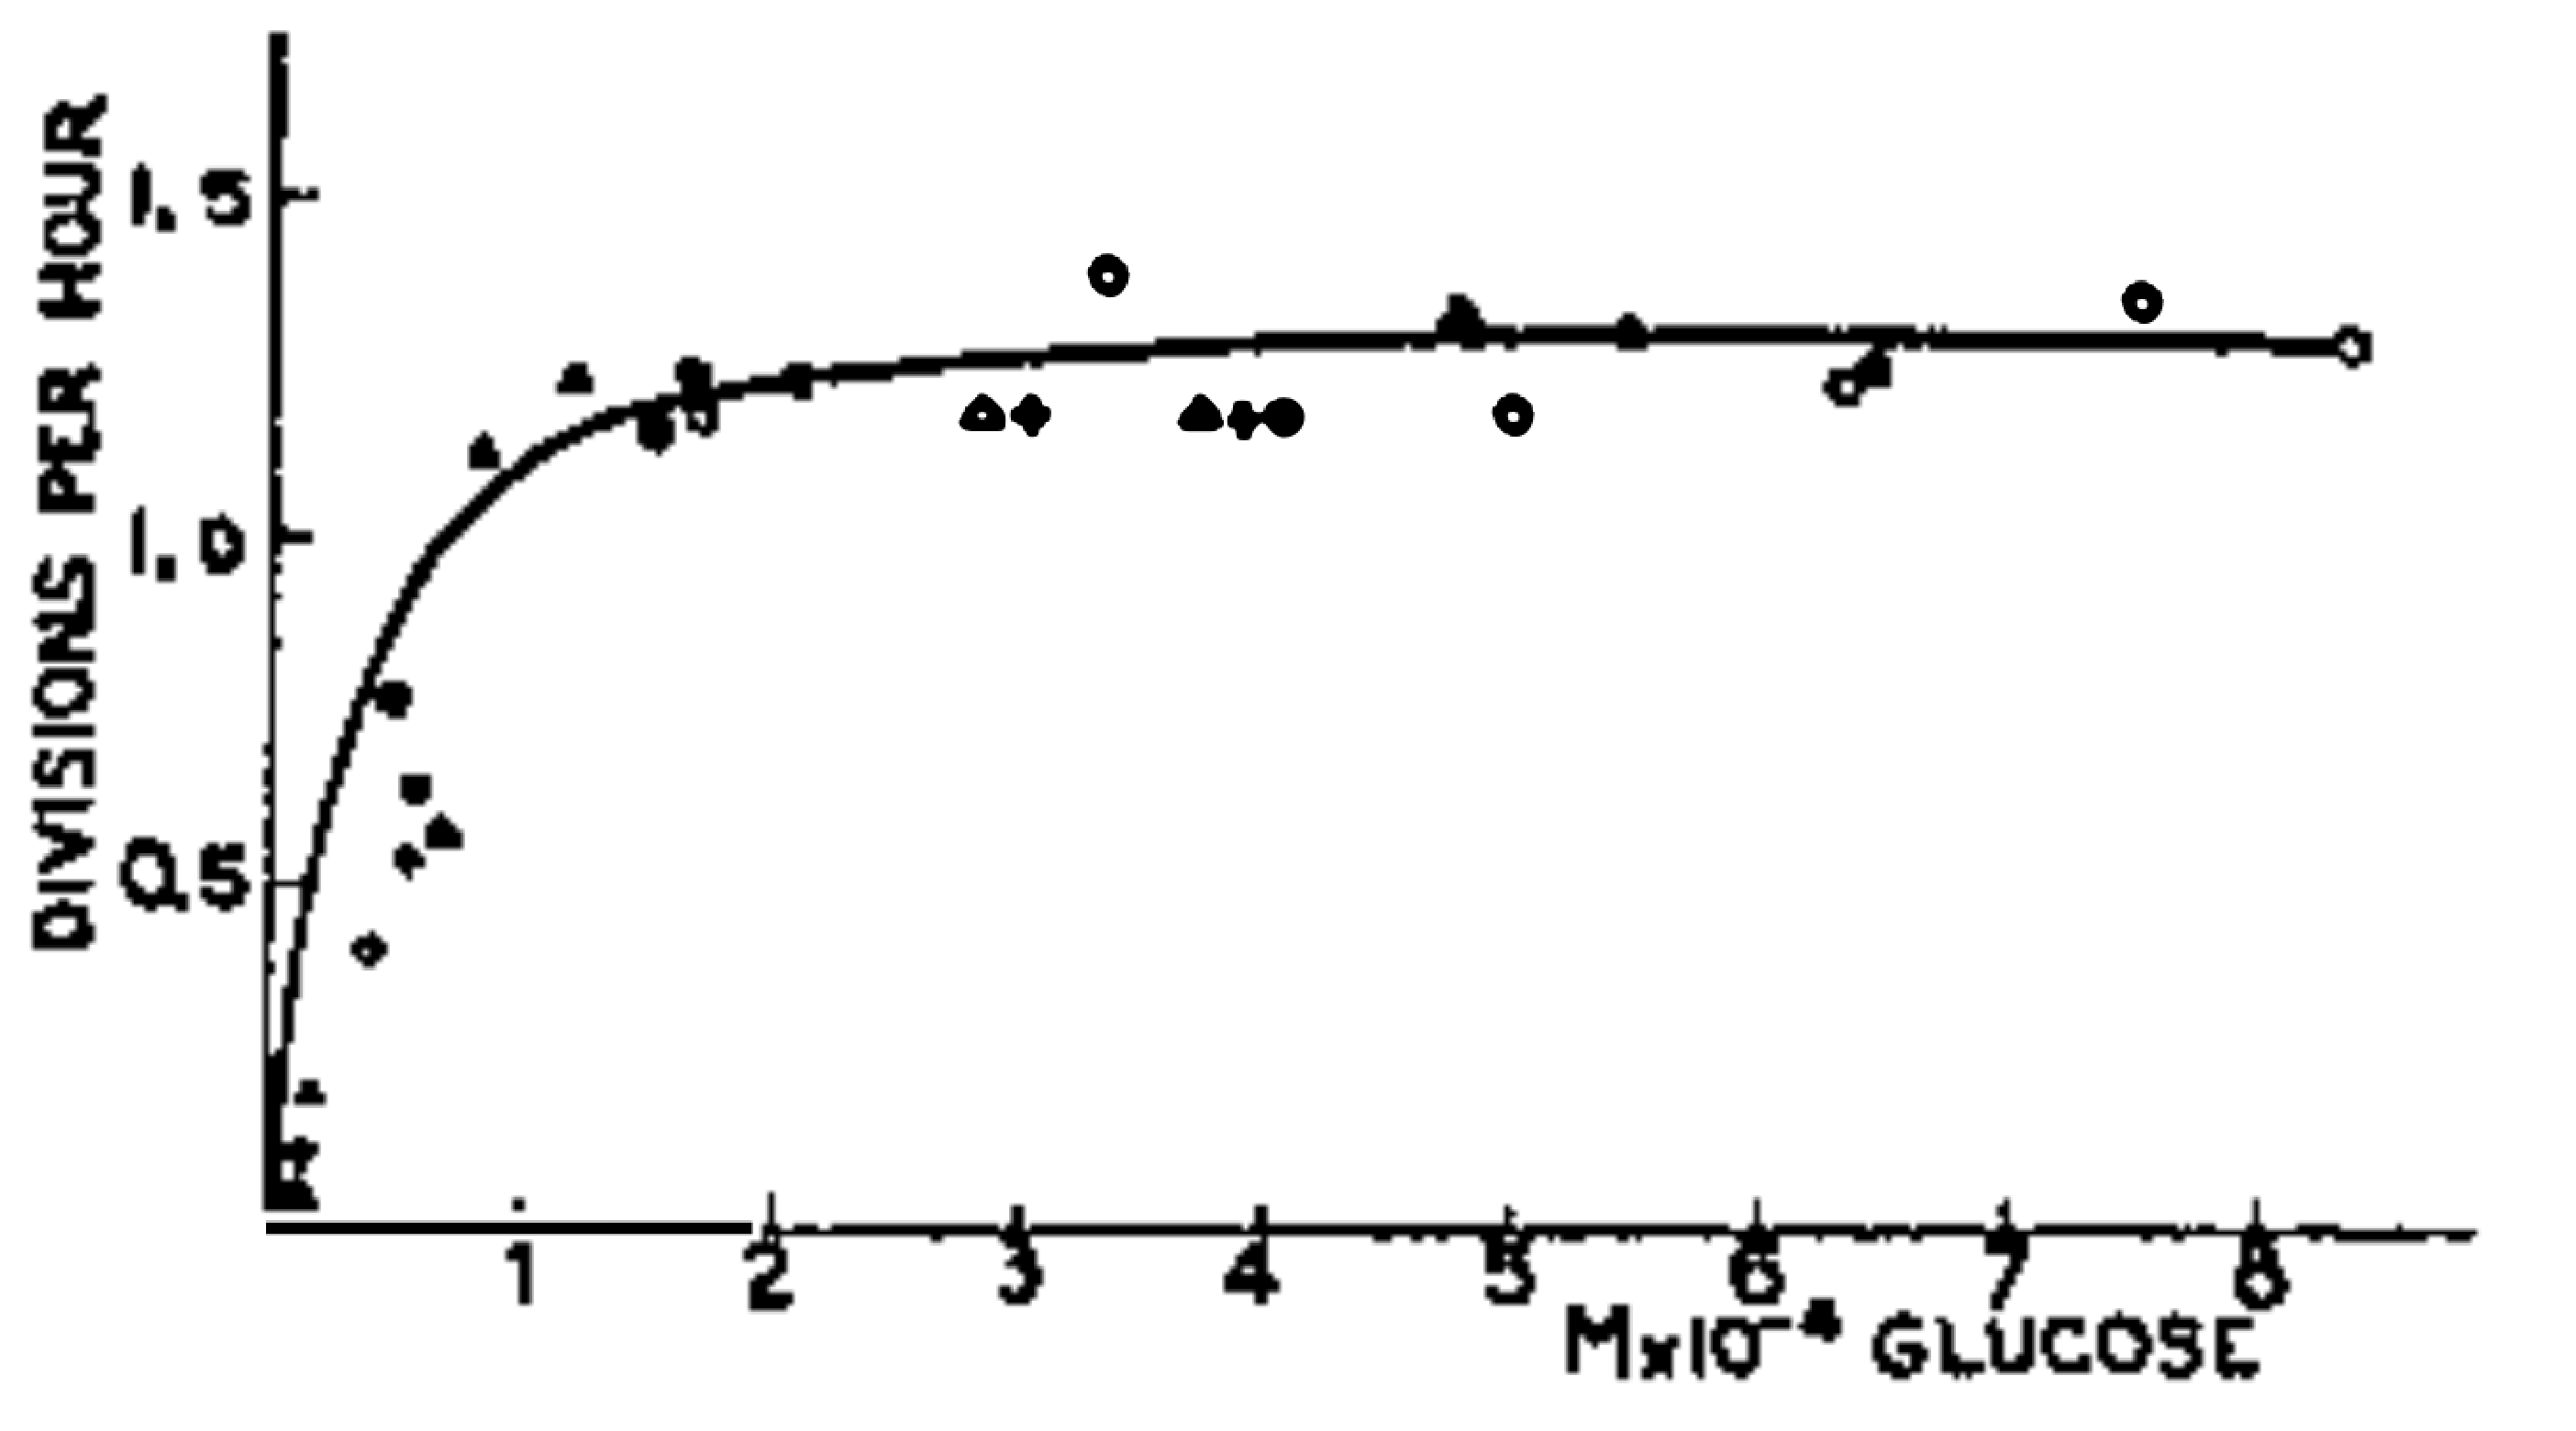
\includegraphics[height=5cm]{./Fig/Chapter1/monod_law.eps}
\caption{
\textbf{Monod law, reproduced from~\cite{monod_growth_1949}.}
Monod has been a pioneer in the formalization of microbial growth into fundamental, coarse-grained relationships.
This figure displays the growth rate (in number of divisions per hour) of \textit{Escherichia coli} in a synthetic minimal medium at 37$^{\circ}$C containing different concentrations of glucose (a common carbon source).
As the concentration of glucose increases, the growth rate of \textit{E. coli} does so by following the hyperbolic relationship described in Eq~\ref{eq:monod_law}.
Solid line is drawn with $\mu_K = 1.35$ div.h\textsuperscript{-1}, and $K_C = 0.22 \cdot 10^{-4}$ mol.L\textsuperscript{-1}.
}
\label{fig:monod_law}
\end{figure}

The production of every component of the cell is controlled by a complex network of regulatory interactions.
But an obvious constraint is that at steady state, the synthesis rate of all individual components must be proportional to the growth rate in order to compensate for growth dilution~\cite{monod_growth_1949}.
Many physiological parameters (like mass of DNA, RNA and proteins) are thus functions of the growth rate alone, regardless of the environmental conditions~\cite{schaechter_dependency_1958,bremer_modulation_1996}.
These so-called growth laws were carefully measured~\cite{bremer_modulation_1996} and are still used today in the quantitative understanding of growth control in microorganisms~\cite{ehrenberg_mediumdependent_2012}.
Recently, the topic was revitalized through the work of Scott \textit{et al}~\cite{scott_bacterial_2011}.
They focused on the ribosome concentration, a physiological parameter that was long known to vary linearly with the growth rate in microorganisms (Fig~\ref{fig:scott_rnaprot}).
By measuring it under different environmental perturbations of the protein synthesis machinery, they built a coarse-grained model describing proteome resource allocation~\cite{scott_emergence_2014}.
It has allowed to show that, whatever the details of the molecular implementation (differing between organisms), this growth law emerges from the underlying principles of robustness and optimization imposed by natural selection, especially growth-rate maximization in every conditions~\cite{scott_emergence_2014}.

\begin{figure}[tb]
\centering
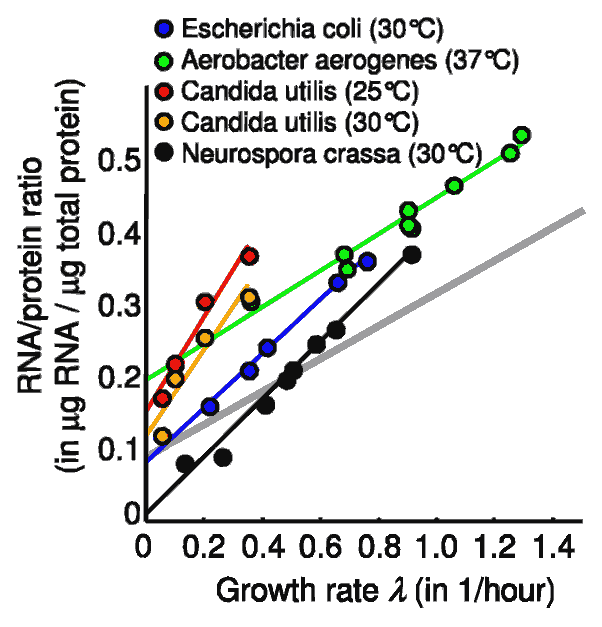
\includegraphics[height=7cm]{./Fig/Chapter1/scott_rnaprot.eps}
\caption{
\textbf{The growth law of ribosomal abundance (figure reproduced from Fig~S1 in~\cite{scott_interdependence_2010}).}
For a variety of carbon nutrients and their corresponding steady-state growth rate, the RNA/protein ratio is linearly correlated with the growth rate, a relation that holds for many species of microorganisms.
This ratio is correlated with the fraction of ribosome-affiliated proteins, and therefore with the relative abundance of ribosomes in the cell.
}
\label{fig:scott_rnaprot}
\end{figure}

\subsection{Static versus dynamical perspective on growth}

The growth laws cited above apply at steady state, where all intensive properties of the cell are time-invariant~\cite{schaechter_microbe_2006,fishov_microbial_1995}.
It means that the properties independent of the cell volume or mass (temperature, concentrations, ...) are constant over time, even though the cell is still growing.
It requires that the components of the cell "increases by the same factor over a time interval", which have motivated the creation of the term balanced growth~\cite{campbell_synchronization_1957}.
Experimentally, this growth scenario has been used as a standard because it improves reproducibility, in that samplings are no longer time-sensitive~\cite{schaechter_microbe_2006}.
It can be easily achieved in the laboratory either in continuous culture, where the substrate is continually supplied, or in batch conditions if the substrate is in high excess (Fig~\ref{fig:growth_curve}).
This approach has been beneficial to mathematical modeling because considering the system at steady state reduces the complexity of the underlying dynamical systems, allowing to build and analyze huge genome-scale models that encapsulate the enzymatic diversity of living cells~\cite{orth_what_2010}.

\begin{figure}[p]
\centering
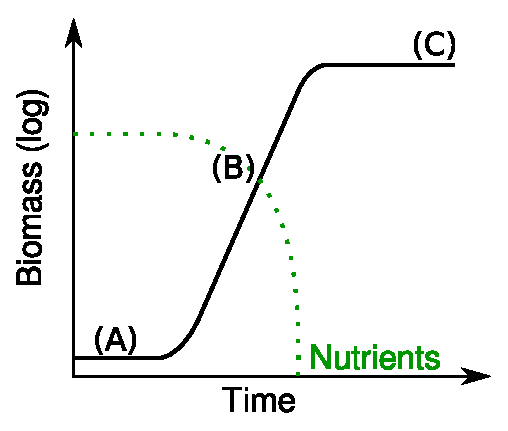
\includegraphics[height=6cm]{./Fig/Chapter1/growth_curve.eps}
\caption{
\textbf{The different phases of a typical growth curve}.
During a typical batch growth scenario, biomass accumulates (black thick line) whereas nutrients are consumed until depletion (green dashed line)~\cite{schaechter_microbe_2006}.
(A) The lag phase, a variable period of time during which the organism adapt to the new medium~\cite{swinnen_predictive_2004}.
It is hardly reproducible and can depends on the pre-culturing history of the strain~\cite{ng_damage_1962,dufrenne_effect_1997,shaw_effect_1967}, the magnitude and the rate of the change between the past and present environments~\cite{mcmeekin_predictive_2002}, and other hard-to-control environmental conditions~\cite{cheroutre-vialette_application_2002}.
(B) The steady-state (or balanced-growth) phase which is characterized by an exponential production of biomass.
It presents constant and reproducible characteristics which has made it a standard for microbial growth studies~\cite{schaechter_microbe_2006}.
This phase can be extended for hundreds of generations by the constant addition of fresh medium (continuous culture)~\cite{wang_robust_2010}.
As represented here, nutrients are quickly depleted in batch conditions, which does not allow to maintain steady-state growth for a long period of time.
(C) The stationary phase, after the depletion of the limited nutrient in the medium~\cite{chubukov_environmental_2014,schaechter_microbe_2006}.
In environmental conditions, microorganisms usually encounter poor media and spend most of their time in stationary phase~\cite{mcarthur_microbial_2006,menge_nitrogen_2012,hobbie_microbes_2013}.
Some species which have evolved long-term resistance mechanisms, like sporulation~\cite{stragier_molecular_1996} or cannibalism~\cite{gonzalez-pastor_cannibalism:_2011}, can survive particularly long stationary phases.
}
\label{fig:growth_curve}
\end{figure}

Although balanced growth is convenient from an experimental and theoretical point of view, it is widely admitted that microorganisms rarely encounter this state in nature~\cite{schaechter_microbe_2006}.
Steady-state growth requires stable conditions over a long period of time, but microorganisms live in
environments where the key elements, such as carbon, nitrogen or phosphorus, are quickly depleted by the competitors as soon as they become available~\cite{mcarthur_microbial_2006,menge_nitrogen_2012,hobbie_microbes_2013}.
Why would microorganisms be optimal for a state they have barely encountered during their evolution?
Are we missing something by studying in stable, unchanging conditions, systems that were in fact selected to cope with environmental variations?

\section{Problem statement}

With their beautiful simplicity, growth laws represent an exceptional point of view on microbial life strategies.
But being established at balanced growth might have drawbacks since it is a growth state totally irrelevant to the life-trait history of microorganisms.
How would growth laws be affected in a dynamical context?
Can we still find universal regularities during growth states more relevant to the natural habitat of microorganisms?

Since we lose the inherent advantages of working at steady state, we must confine our problem to keep it tractable.
We then focus on the fundamentals behind resource allocation (the proteome composition growth law), especially the regulation of the abundance of gene expression machinery during the transition between two different growth media.

On the theoretical side, we assess if there exist a universal optimal way to allocate cell resources during growth transitions.
On the experimental side, we monitor the abundance of key macromolecular components in order to get an insight that could be compared with the theoretical predictions.

\section{Related work}

\subsection{Modeling growth of microorganisms}

My recent experience as a teacher taught me that, as of today, a lot of students still choose to study biology in the hope to find a math-free job in science.
They fall from the clouds when you tell them modeling is an important part of a biologist's life.
This misconception usually comes from a bad understanding of what is modeling.
In its general sense, a model depicts and simplifies reality.
Maps, sketches, or pictures satisfy this definition, as do graphs, sets of equations, or even the DNA sequences I store in a text-file on my computer.
Overall, depicting and simplifying reality makes you a modeler, not so much drawing equations on a board.
But this does not change the fact that mathematics are incredible tools for these purposes~\cite{servedio_not_2014,mcgill_calm_2013}.

What makes mathematical modeling so useful in microbial growth studies?
Microbial physiology comes out from the interplay of thousands of chemical reactions that are not necessarily relevant in any given situation.
They usually occur on a short time scale as compared with the organism life span.
They nevertheless have been (and still are) selected by evolutionary processes that occur on long time scales.
These physical limitations strongly impede a full empirical study of growth processes, making sometimes hard to test the most simple verbal hypothesis.
Since they are designed to abstract away complexity, mathematical models are great tools to deal with such limitations.
The overwhelming number of variables and time scales can be dealt with by choosing the correct framework.
When working on a model, growth is abstracted into a world of clearly stated rules, where logical reasoning can be applied~\cite{servedio_not_2014}.
Predictions can be made, "unpacked" into our real world, and confronted with experimental testing.
In that sense, modeling is at the core of the scientific method~\cite{mcgill_calm_2013}.
This could explain why mathematical modeling has been extensively applied to microbial growth studies, creating a diversity a modeling framework.

For an increasing number of microorganisms, we are now able to draw quasi-exhaustive maps of their inner metabolic reactions.
This has been made possible by the advances on genome reconstruction, which are easier and cheaper to accomplish every passing year.
But making sense of these data proved to be even more challenging.
Which reactions are important, and in which conditions?
How will a metabolic network react to perturbations?
Can we predict its evolution in a given environment?
When dealing with genome-scale metabolic networks, one is challenged by the number of metabolites and possible reactions (e.g. the most recent genome-scale reconstruction of \textit{E. coli} metabolism contains "1366 genes, 2251 metabolic reactions, and 1136 unique metabolites"~\cite{orth_comprehensive_2011}).
More importantly, while progress in genomic made possible such reconstructions, measuring precise \textit{in-vivo} kinetic parameters for all these reactions still represents a technological bottleneck~[citation?].
Nevertheless, a modeling framework is specifically designed to deal with such limitations: constraint-based modeling.
This framework abstracts away the unknown kinetics and represents the metabolic maps as a flux map on which physico-chemical constraints can be applied, e.g. steady-state, compartmentalization, mass conservation, molecular crowding, and thermodynamic directionality~\cite{ebrahim_cobrapy_2013}.
Candidates for the flux distribution are obtained by optimizing the system towards an objective function, which usually represents growth rate for microorganisms.
One can find a lot of derivatives of this framework, but its the Flux Balance Analysis that renewed interest into it [citation review ?].
\textbf{[Need some key results that were obtained, or this paragraph makes no sense].}
Note that such a level of abstraction necessarily has its drawbacks, e.g. the definition of the objective function, the difficulty to work in dynamic or implement information on the metabolic regulations [citation?].

The ever-growing available data on metabolic networks can also be used to make large kinetic models.
For the reasons we stated above, we expect these models to be inherently limited in scope.
It means that the modeler has to be extremely careful since he or she injects its knowledge about what might be important in the system, for the question he or she tries to solve.
They are however more flexible, in the sense that one can easily make interplay different level of regulations.
\textit{[Present the work of Klumpp, Kremling, Sauer, whole model of genitallium, etc]
}\textit{Especially the work of Klumpp, Kremling, Sauer, etc, also the whole model of genitallium.
Biggest problem is the lack of parameter values, and some huge trouble with identifiability.
They have medium to large scope (increasing), highly detailed granularity and deal with the mathematical complexity via the computational power via the use of huge quantity of data.}

Another approach has shown successful in understanding some aspects of growth behaviors of microorganisms.
By applying a high level of abstraction on how the cell functions, it becomes easy to compare data about different species and to uncover general evolutionary principles that are independent of the specific implementation in each organism.
Best examples of this approach are the empirical growth laws of ribosomal abundance~\cite{scott_bacterial_2011,scott_interdependence_2010,scott_emergence_2014}, or the proof-of-concept explanation of overflow metabolism~\cite{molenaar_shifts_2009} that were described in section~\ref{sec:context} of this introduction.
It is also the preferred approach when one wants to broaden its access to mathematical tools~\cite{vandenberg_optimal_1998}, most of them being unhelpful with the high dimensionality of biological models.
As we will describe in section~\ref{sec:approach}, this represents the modeling strategy that was used in this thesis.

Coarse-grained models have also been helpful to understand the process by which microorganisms switch to inefficient metabolic pathways when growing at high nutrient availability.
Since nutrients are not used at their full potential given the environmental conditions, this widespread growth strategy apparently leads to energy waste, ~\cite{molenaar_shifts_2009} (Fig~\ref{fig:molenaar_overflow}).
Originally called the Crabtree effect when first observed in \textit{Saccharomyces cerevisiae}~\cite{dijken_kinetics_1993} and overflow metabolism when later found in \textit{E. coli}~\cite{vemuri_overflow_2006}, it has also been called the Warburg effect in many types of tumor cells~\cite{mckeehan_glycolysis_1982,hsu_cancer_2008}.
Molenaar \textit{et al} showed that this phenomenon simply results from the underlying principle of growth rate maximization, in particular the trade-off between the cost of enzyme synthesis and the pathway efficiency~\cite{molenaar_shifts_2009}.
Like traders, bacteria distribute their resources between different beneficiaries, and tend to do so in a way that maximizes returns on investments.

\begin{figure}[tb]
\centering
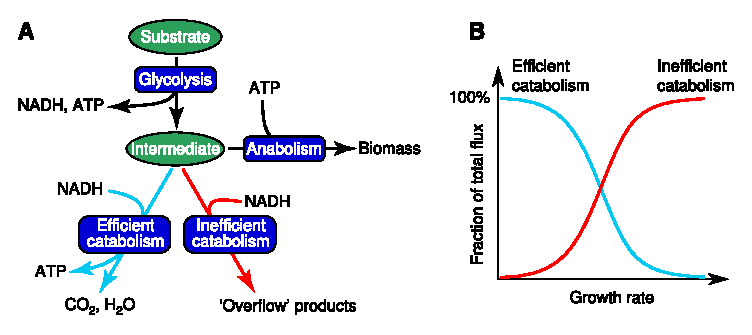
\includegraphics[width=\textwidth]{./Fig/Chapter1/molenaar_overflow.eps}
\caption{
\textbf{The strategy of overflow metabolism, reproduced from~\cite{molenaar_shifts_2009}.}
When increasing the concentration of substrate, the metabolism of microorganisms switches toward the use of inefficient pathways.
This paradoxical behavior does in fact maximize the growth rate if we take into account the costs and benefits of enzyme synthesis, in particular the fact that pathways for inefficient catabolism are shorter and therefore cheaper to produce.
(A) Simple view of microbial metabolism, with the two competing efficient and inefficient pathways.
(B) The switching from efficient to inefficient catabolism when the concentration of nutrients, and hence the growth rate, increases.
}
\label{fig:molenaar_overflow}
\end{figure}

\subsection{Measuring growth of microorganisms}

\textbf{Either to build models or test their predictions, data on microbial growth have to be acquired.}
Measuring growth = measuring biomass accumulation, over time, and get relevant information on the cell inner state.
We have a lot of data on this.

\textbf{Measuring population-wide parameters is convenient and provides robust data.}
Population measurement is easy to implement, and some things can only be measured at the population level (so far).
But small unsynchronized effects can be hidden since we mostly work with the mean.
Despite most of the knowledge we have on microorganism growth are from population measurements, like the RNA/DNA/etc ratios, the growth laws, etc.
Extensive work of Bremmer and Dennis.
Big discoveries of the last decades that rely on population measurements ? (cite 2 or 3)

\textbf{Single-cell measurements give access to data and behaviors that are hidden at the population level.}
Single-cell measurements lay on technologies like microscopy, fluorescence, FACS...
More interesting since we can use fluorescence to not just look at the cell but also measure interesting parameters (like gene expression) at the single-cell level.
Information on the localisation of DNA, ribosomes [Bakshi].
Variability in physiology, persistors, antibiotics resistance, etc [citations]

\textbf{Batch growing conditions are convenient and close to the natural conditions of bacteria, but they raise several problems.}
Both approaches can be performed either in batch or continuous conditions.
Batch conditions is the most straight forward in lab: you put sugar in a flask, they grow until nutrient is depleted.
Implemented in flash or petri-microscopy.
Resist to contamination.
It is close to natural conditions, and industrial conditions.
Has even been used to study long-term evolution of E. coli.
But the system is poorly control, mostly because the history of the cells play a huge role in the waking process.

\textbf{Continous cultures allow to precisely control the growing conditions.}
Continuous culture consists into constantly providing nutrients to a culture, and maintaining it in a steady-state for a long time.
Implemented in bioreactor [citation] or microfluidic devices [mother machine citation].
Sensible to contaminations so hard to maintained (that's why industry ignore it so far).
Does not correspond to natural conditions but the system is fully controlled: perturbations can be applied and a lot of parameters can be monitored.
Possibility to let the cell long-enough in steady state to "forget" strain history.
Most suitable if one need to have full control on its system.

\textbf{In all these practical conditions, one can choose to either measure cells at steady-state or in dynamic.}
Finally, most of the work cited above are based on steady-state studies.
But there are also work in dynamic.
Levy showed that... in yeast.
Alon in Coli.
After decades working at steady-state, Bremmer and Dennis argued we should measure things during transitions.
de Jong / Gerosa showed that the gene expression machinery has its own dynamic that should be taken into account when measuring gene expression.
The evolutionary relevance of growth transitions has been emphasized in numerous others studies [citations lag phase, last generation before stationary, ...].

\section{Approach}
\label{sec:approach}

We first tackle the problem of creating a mathematical framework for studying environmental transitions.
\textit{Building upon the work cited above, we create a simple self-replicator model that allocate resources between two sections.}

The goal is to identify what would be an ideal transition.
\textit{We all have an intuitive idea of what should be a good transition: it should be fast, robust, etc... But it is unclear how this relates to the fitness factor that shaped the regulatory mechanisms of microorganisms.}

We describe dynamical optimality by using optimal control theory.
\textit{Brieve explanation about optimal control theory and how it is used in economic or engineering to optimize or understant dynamical processes.}

All of this is described in chapter 2.

Then, after we know what to look for, we try to actually measure how resource allocation occurs in a model organism: \textit{Escherichia coli}.
\textit{We justify the use of coli and introduce the gene expression fluorescent reporter.
We made a strain with fluorescent ribosomes, and studied our experimental framework in different transitions, at the population and the single cell level.
We justify the use of both by the fact that population is easy for "screening", and single cell allow for a better resolution and take care of the "desynchronization" biais that could occur.}

This, is described in chapter 3.